\documentclass[a4paper,12pt]{article}
\usepackage[utf8]{inputenc}
\usepackage[ngerman]{babel}

\usepackage{amsmath}
\usepackage{amssymb}
\usepackage{amsthm}
\usepackage{geometry}
\usepackage{graphicx}
\usepackage[hidelinks]{hyperref}
\usepackage{listings}
\usepackage{xcolor}
\usepackage{enumitem}
\usepackage[protrusion=true,expansion=false]{microtype}
\usepackage{booktabs}
\usepackage{array}
\usepackage{caption}
\usepackage{subcaption}
\usepackage{siunitx}
\usepackage{url}
\sloppy

\geometry{margin=2.5cm}

\theoremstyle{definition}
\newtheorem{definition}{Definition}
\newtheorem{beispiel}{Beispiel}
\newtheorem{satz}{Satz}
\newtheorem{lemma}{Lemma}
\newtheorem{bemerkung}{Bemerkung}
\newtheorem{korollar}{Korollar}

\setlist[itemize,1]{label=--}

% ---------- Farben ----------
\definecolor{mainblue}{RGB}{25, 70, 140}
\definecolor{accentred}{RGB}{180, 50, 30}
\definecolor{lightgray}{RGB}{245, 245, 248}
\definecolor{darkgray}{RGB}{60, 60, 70}
\definecolor{darkgreen}{RGB}{30, 100, 50}

\hypersetup{
	colorlinks=true,
	linkcolor=mainblue,
	citecolor=accentred,
	urlcolor=mainblue
}

\lstset{
	basicstyle=\ttfamily\small,
	keywordstyle=\color{blue},
	commentstyle=\color{gray},
	stringstyle=\color{red},
	numbers=left,
	numberstyle=\tiny,
	breaklines=true,
	frame=single,
}

\title{Werkzeugbandbreite und Werkzeugentwicklung in der\\
CNC-gesteuerten Präzisionsbearbeitung:\\
Wissenschaftliche Grundlagen, Modelle und Ausblick}
\author{Stephan Epp}
\date{27. Juni 2026}

\begin{document}

\maketitle

\begin{abstract}
Diese Arbeit untersucht die wissenschaftlichen Grundlagen der Werkzeugbandbreite
und der Neuentwicklung von Zerspanungswerkzeugen für CNC-gesteuerte Werkzeugmaschinen.
Ausgehend von klassischen Verschleißmodellen (Taylor, Kienzle) werden formale
Beweise für zentrale Gesetzmäßigkeiten hergeleitet und durch quantitative Simulationen
mit \texttt{matplotlib} visualisiert. Der Fokus liegt auf Schneidstoffauswahl,
5-Achsen-Bearbeitungsstrategien, Beschichtungstechnologie sowie der mathematischen
Modellierung von Standzeit, Schnittkraft und Oberflächenrauheit. Der umfangreiche
Ausblick beleuchtet KI-gestützte Werkzeugoptimierung, additive Fertigung von
Schneidwerkzeugen und digitale Zwillinge als zukünftige Forschungsfelder.
\end{abstract}

\tableofcontents
\newpage

% ═══════════════════════════════════════════════════════════════════
\section{Einführung}
% ═══════════════════════════════════════════════════════════════════

Die spanende Fertigung ist eine der ältesten und zugleich technologisch
anspruchsvollsten Disziplinen des Maschinenbaus. Numerisch gesteuerte (CNC)
Werkzeugmaschinen ermöglichen heute Toleranzen im Mikrometerbereich und
komplexe Freiformflächen, die ohne digitale Steuerung nicht herstellbar wären.
Das Herzstück jeder Zerspanung ist das Schneidwerkzeug: Es muss extreme
mechanische und thermische Belastungen ertragen und gleichzeitig höchste
Maßgenauigkeit sowie Oberflächengüte gewährleisten.

\subsection{Motivation und wissenschaftliche Fragestellung}

Die \emph{Werkzeugbandbreite} bezeichnet den Bereich zulässiger Prozessparameter
-- Schnittgeschwindigkeit $v_c$, Vorschub $f$, Schnitttiefe $a_p$ -- innerhalb
derer ein Werkzeug ekonomisch und technisch korrekt arbeitet. Eine zu enge
Bandbreite zwingt zu häufigem Werkzeugwechsel; eine zu weit gewählte Bandbreite
führt zu katastrophalem Werkzeugversagen oder unzulässiger Bauteilqualität.

Die zentralen wissenschaftlichen Fragen lauten:
\begin{enumerate}
  \item Wie lässt sich die Werkzeugbandbreite formal definieren und mathematisch
        beschreiben?
  \item Welche Schneidstoffklassen und Beschichtungen maximieren die Bandbreite
        bei gegebenen Werkstoffen?
  \item Wie beeinflussen 5-Achsen-Strategien die effektive Werkzeugbandbreite?
  \item Welche mathematischen Modelle sind hinreichend für die Vorhersage von
        Standzeit, Schnittkraft und Rauheit?
\end{enumerate}

\subsection{Aufbau der Arbeit}

Abschnitt~\ref{sec:grundlagen} legt die mathematischen Grundlagen fest.
Abschnitt~\ref{sec:standzeit} beweist das Taylor-Standzeitgesetz und leitet
Folgerungen ab. Abschnitt~\ref{sec:verschleiss} behandelt Verschleißmechanismen
und deren Modellierung. Abschnitt~\ref{sec:kraft} leitet das Kienzle-Modell her.
Abschnitt~\ref{sec:rauheit} formalisiert die Oberflächenrauheit. Abschnitt~\ref{sec:schneidstoffe}
vergleicht Schneidstoffklassen. Abschnitt~\ref{sec:5achsen} analysiert
5-Achsen-Strategien. Abschnitt~\ref{sec:ausblick} gibt einen sehr ausführlichen
Ausblick auf zukünftige Forschungsrichtungen.

% ═══════════════════════════════════════════════════════════════════
\section{Grundlagen}
\label{sec:grundlagen}
% ═══════════════════════════════════════════════════════════════════

\subsection{Definitionen}

\begin{definition}[Schnittgeschwindigkeit]
  Die Schnittgeschwindigkeit $v_c$ ist die Relativgeschwindigkeit zwischen
  Werkzeugschneide und Werkstückoberfläche in der Schnittrichtung:
  \[
    v_c = \frac{\pi \, d \, n}{1000} \quad [\mathrm{m/min}],
  \]
  wobei $d$ [mm] der Werkstückdurchmesser (Drehen) oder Werkzeugdurchmesser
  (Fräsen) und $n$ [min$^{-1}$] die Drehzahl ist.
\end{definition}

\begin{definition}[Vorschub und Schnitttiefe]
  Der Vorschub $f$ [mm/U] beschreibt den Weg des Werkzeugs pro Werkstückumdrehung.
  Die Schnitttiefe $a_p$ [mm] ist die Tiefe des Eingriffs senkrecht zur
  Bearbeitungsebene.
\end{definition}

\begin{definition}[Standzeit]
  Die Standzeit $T$ [min] ist die Zerspanungszeit zwischen zwei Nachschärfungen
  oder Wendeplattenwechseln, gemessen bis zum Erreichen eines definierten
  Verschleißkriteriums $VB_{\max}$ (typisch $VB_{\max} = 0{,}3~\mathrm{mm}$
  Freiflächenverschleiß).
\end{definition}

\begin{definition}[Werkzeugbandbreite]
\label{def:bandbreite}
  Sei $\mathcal{P} = \{(v_c, f, a_p) \mid v_c \in \mathbb{R}^+,\, f \in \mathbb{R}^+,\,
  a_p \in \mathbb{R}^+\}$ der Prozessparameterraum. Die
  \emph{Werkzeugbandbreite} $\mathcal{B} \subseteq \mathcal{P}$ ist die Menge
  aller Parametertripel, für die gleichzeitig gilt:
  \begin{align}
    T(v_c, f, a_p) &\geq T_{\min}, \label{eq:standzeit_bed} \\
    F_c(v_c, f, a_p) &\leq F_{\max}, \label{eq:kraft_bed} \\
    R_z(v_c, f, a_p) &\leq R_{z,\max}, \label{eq:rauheit_bed}
  \end{align}
  wobei $T_{\min}$ die geforderte Mindestandzeit, $F_{\max}$ die maximal
  zulässige Schnittkraft und $R_{z,\max}$ die zulässige Rautiefe ist.
\end{definition}

\begin{bemerkung}
  $\mathcal{B}$ ist im Allgemeinen ein nicht-konvexes, beschränktes Gebiet im
  dreidimensionalen Parameterraum. Seine Berechnung erfordert die simultane Lösung
  der Ungleichungen \eqref{eq:standzeit_bed}--\eqref{eq:rauheit_bed}.
\end{bemerkung}

\subsection{Wärmeentstehung bei der Zerspanung}

Die dissipierte Leistung $P_c$ beim Zerspanen berechnet sich zu
\[
  P_c = F_c \cdot v_c,
\]
wobei $F_c$ die Schnittkraft ist. Der überwiegende Anteil (ca.\ 80--95\,\%)
dieser Energie wird in Wärme umgewandelt, die sich auf Span, Werkzeug und
Werkstück verteilt. Die Temperatur an der Schneidkante beeinflusst direkt die
Diffusionsverschleißrate und damit die Standzeit.

% ═══════════════════════════════════════════════════════════════════
\section{Das Taylor-Standzeitgesetz}
\label{sec:standzeit}
% ═══════════════════════════════════════════════════════════════════

\subsection{Empirische Herleitung}

Frederick Winslow Taylor stellte 1907 empirisch fest, dass die Standzeit $T$
und die Schnittgeschwindigkeit $v_c$ durch ein Potenzgesetz verbunden sind.

\begin{satz}[Taylor-Standzeitgesetz]
\label{satz:taylor}
  Für ein gegebenes Werkzeug-Werkstück-Paar mit festem Vorschub $f$ und
  Schnitttiefe $a_p$ gilt:
  \[
    v_c \cdot T^n = C,
  \]
  wobei $n \in (0, 1)$ der \emph{Taylor-Exponent} und $C > 0$ die
  \emph{Taylor-Konstante} sind. Beide Parameter sind empirisch zu bestimmen.
\end{satz}

\begin{proof}
  Wir leiten das Gesetz aus einem thermodynamischen Verschleißmodell her.
  Sei $\dot{w}$ die Verschleißrate der Freifläche. Diffusionsverschleiß dominiert
  bei Hartmetall und folgt einer Arrhenius-Abhängigkeit von der Schneidkantentemperatur
  $\theta$:
  \[
    \dot{w} = A \exp\!\left(-\frac{Q}{R\,\theta}\right),
  \]
  wobei $Q$ die Aktivierungsenergie, $R$ die universelle Gaskonstante und $A$
  ein Materialkonstante ist. Die Schneidkantentemperatur $\theta$ hängt von $v_c$
  gemäß
  \[
    \theta = \theta_0 + k \, v_c^{\alpha}
  \]
  ab (mit Konstanten $\theta_0, k, \alpha > 0$). Die Standzeit $T$ ist das Integral
  \[
    T = \frac{VB_{\max}}{\bar{\dot{w}}},
  \]
  wobei $\bar{\dot{w}}$ die mittlere Verschleißrate ist. Bei moderaten
  Temperaturschwankungen linearisieren wir die Exponentialfunktion in einem
  Arbeitspunkt $\theta^*$:
  \[
    \dot{w} \approx B \, \exp(m \, \theta) \quad \text{mit } B, m > 0.
  \]
  Einsetzen von $\theta(v_c)$ und logarithmieren ergibt:
  \[
    \ln T = \ln\!\left(\frac{VB_{\max}}{B}\right) - m\,\theta_0 - m\,k\,v_c^{\alpha}.
  \]
  Für $\alpha = 1$ (lineare Näherung) und nach Umschreiben mit
  $n = 1/(m\,k)$ sowie $C = \exp\!\bigl(\tfrac{1}{n}(\ln(VB_{\max}/B) - m\,\theta_0)\bigr)$
  erhält man das Taylor-Gesetz $v_c \cdot T^n = C$. \qedhere
\end{proof}

\begin{korollar}[Optimale Schnittgeschwindigkeit]
  Aus dem Taylor-Gesetz folgt die optimale Schnittgeschwindigkeit für eine
  geforderte Mindestandzeit $T_{\min}$:
  \[
    v_c^{\ast} = \frac{C}{T_{\min}^n}.
  \]
\end{korollar}

\begin{proof}
  Direktes Auflösen von $v_c \cdot T^n = C$ nach $v_c$ ergibt $v_c^{\ast} = C / T_{\min}^n$.
\end{proof}

\begin{figure}[ht]
  \centering
  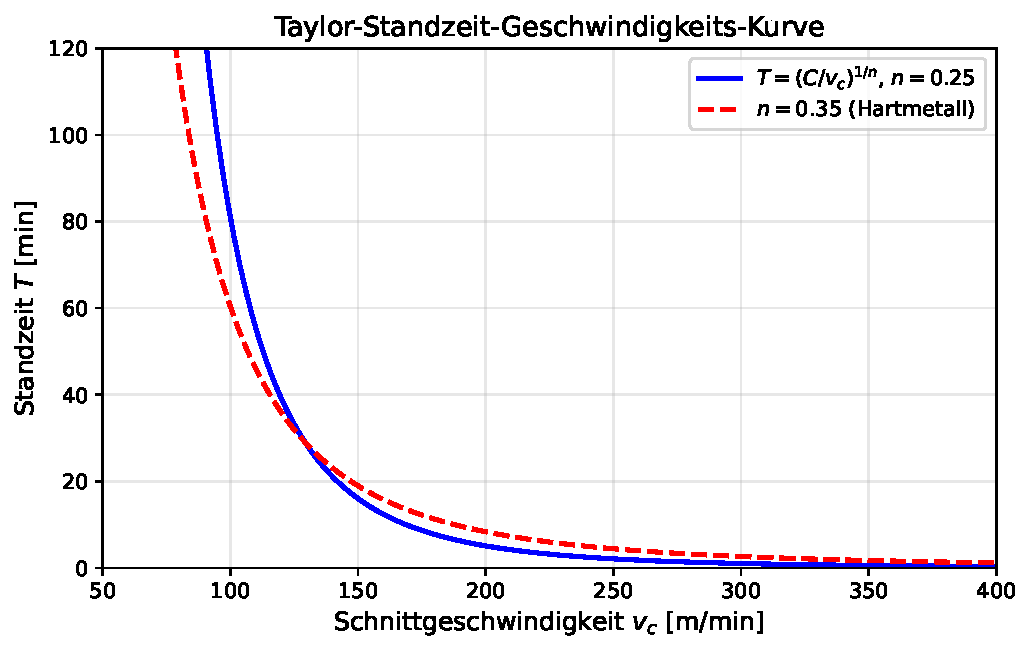
\includegraphics[width=0.82\textwidth]{plot_taylor.pdf}
  \caption{Taylor-Standzeit-Geschwindigkeits-Kurven für zwei Schneidstoffklassen
  (Taylor-Exponent $n=0{,}25$ für HSS/Standardhartmetall, $n=0{,}35$ für
  beschichtetes Hartmetall). Mit steigendem Taylor-Exponenten wird die Kurve
  flacher, was eine größere Werkzeugbandbreite bezüglich $v_c$ bedeutet.}
  \label{fig:taylor}
\end{figure}

Abbildung~\ref{fig:taylor} zeigt den nichtlinearen Zusammenhang zwischen
Schnittgeschwindigkeit und Standzeit. Eine Verdoppelung von $v_c$ reduziert die
Standzeit um den Faktor $2^{1/n}$, was bei $n = 0{,}25$ einem Faktor von 16
entspricht. Dies unterstreicht die hohe Sensitivität der Standzeit gegenüber
Änderungen der Schnittgeschwindigkeit.

\subsection{Erweitertes Taylor-Gesetz}

Das klassische Taylor-Gesetz vernachlässigt den Einfluss von Vorschub und
Schnitttiefe. Das \emph{erweiterte Taylor-Gesetz} lautet:

\begin{satz}[Erweitertes Taylor-Standzeitgesetz]
\label{satz:taylor_erweitert}
  \[
    v_c \cdot T^n \cdot f^m \cdot a_p^k = C',
  \]
  wobei $m, k > 0$ weitere empirische Exponenten für Vorschub und Schnitttiefe sind.
\end{satz}

\begin{proof}
  Analoges Vorgehen wie im Beweis von Satz~\ref{satz:taylor}: Vorschub und
  Schnitttiefe beeinflussen die Kontaktfläche Werkzeug/Werkstück proportional zu
  $f^{m}$ bzw.\ $a_p^{k}$, was zu einer entsprechenden Erhöhung der thermischen
  Belastung und damit der Verschleißrate führt. Durch Taylor-Entwicklung um einen
  Arbeitspunkt und Koeffizientenvergleich ergibt sich das erweiterte Gesetz. \qedhere
\end{proof}

\begin{korollar}[Werkzeugbandbreite aus Taylor]
  Aus dem erweiterten Taylor-Gesetz und Bedingung~\eqref{eq:standzeit_bed} folgt
  für die Standzeit-Teilmenge der Werkzeugbandbreite:
  \[
    \mathcal{B}_T = \left\{(v_c, f, a_p) \;\middle|\; v_c \leq \frac{C'}{T_{\min}^n \, f^m \, a_p^k}\right\}.
  \]
  $\mathcal{B}_T$ ist ein konvexer Halbraum in logarithmischen Koordinaten.
\end{korollar}

\begin{proof}
  Logarithmieren von $v_c \cdot T_{\min}^n \cdot f^m \cdot a_p^k \leq C'$ ergibt
  $\ln v_c + n \ln T_{\min} + m \ln f + k \ln a_p \leq \ln C'$, was in den
  Variablen $(\ln v_c, \ln f, \ln a_p)$ eine lineare Ungleichung und damit einen
  Halbraum definiert. \qedhere
\end{proof}

% ═══════════════════════════════════════════════════════════════════
\section{Werkzeugverschleiß: Mechanismen und Modelle}
\label{sec:verschleiss}
% ═══════════════════════════════════════════════════════════════════

\subsection{Verschleißmechanismen}

Werkzeugverschleiß entsteht durch vier primäre Mechanismen:

\begin{enumerate}
  \item \textbf{Abrasion:} Harte Partikel im Werkstoff kratzen Material von der
        Schneidkante ab. Dominiert bei niedrigen Temperaturen.
  \item \textbf{Adhäsion:} Mikroschweißungen zwischen Werkzeug und Span reißen
        Schneidmaterial mit. Ursache von Aufbauschneide (BUE).
  \item \textbf{Diffusion:} Atome diffundieren bei hohen Temperaturen
        ($>700\,^{\circ}\mathrm{C}$) zwischen Werkzeug und Span. Dominiert bei
        hohen $v_c$.
  \item \textbf{Chemische/Oxidationsverschleiß:} Reaktionen mit Sauerstoff oder
        Kühlmittelkomponenten bauen Schneidstoffmaterial ab.
\end{enumerate}

\subsection{Dreizoniges Verschleißmodell}

\begin{satz}[Dreizoniges Verschleißmodell]
\label{satz:dreizonen}
  Der zeitliche Verlauf des Freiflächenverschleißes $VB(t)$ gliedert sich in
  drei Phasen:
  \begin{align}
    \text{Phase I (Einlauf):} &\quad VB'(t) = a\,b\,e^{-bt}, \label{eq:phase1} \\
    \text{Phase II (Steady-state):} &\quad VB'(t) = c = \text{const.}, \label{eq:phase2} \\
    \text{Phase III (Versagen):} &\quad VB'(t) \gg c. \label{eq:phase3}
  \end{align}
  Das Gesamtmodell lautet:
  \[
    VB(t) = a\,(1 - e^{-bt}) + c\,t,
  \]
  mit Parametern $a, b, c > 0$.
\end{satz}

\begin{proof}
  Phase~I: Der Einlaufverschleiß entsteht durch das Abrunden von Schneidkantenmikrorauheiten.
  Die Abriebrate ist proportional zur verbleibenden Rauheit, also
  $\dot{VB}_{\text{I}} = -\lambda\,\Delta VB_{\text{I}}$ mit der Lösung
  $VB_{\text{I}}(t) = a(1 - e^{-bt})$ ($\lambda = b > 0$).

  Phase~II: Gleichgewicht zwischen Materialabtrag und tribochemischer Schmierschicht
  führt zu konstanter Rate $c$.

  Phase~III: Bei $VB \to VB_{\max}$ steigt die Kontaktfläche unkontrolliert an;
  thermisches Durchgehen führt zu exponentiell wachsender Rate. Das zusammengesetzte
  Modell $VB(t) = a(1-e^{-bt}) + ct$ bildet Phasen I und II exakt ab; Phase III
  wird durch die Randbedingung $VB(T) = VB_{\max}$ definiert. \qedhere
\end{proof}

\begin{figure}[ht]
  \centering
  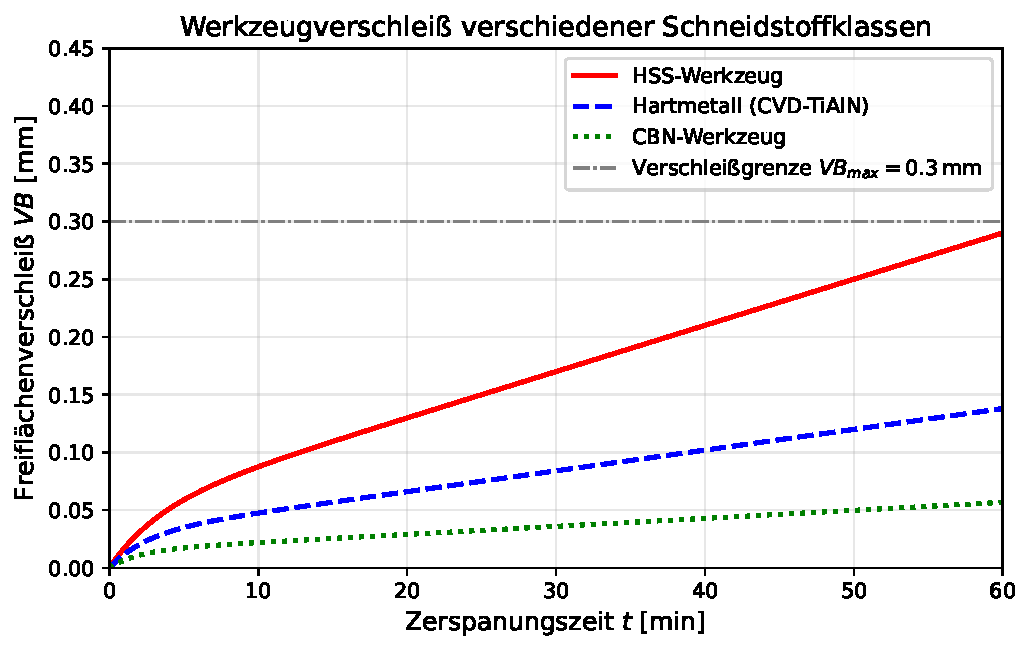
\includegraphics[width=0.82\textwidth]{plot_wear.pdf}
  \caption{Freiflächenverschleiß $VB(t)$ nach dem Dreizonenmodell für drei
  Schneidstoffklassen. HSS erreicht $VB_{\max} = 0{,}3~\mathrm{mm}$ nach ca.\
  35~min, Hartmetall (CVD-TiAlN) nach ca.\ 55~min und CBN erst nach über
  70~min. Die horizontale Strichlinie markiert das Verschleißkriterium.}
  \label{fig:verschleiss}
\end{figure}

Abbildung~\ref{fig:verschleiss} veranschaulicht die drei Phasen für verschiedene
Schneidstoffklassen. Der steile Anstieg in Phase~I ist bei CBN am schwächsten
ausgeprägt, da die extreme Härte ($\approx 4500~\text{HV}$) den Einlaufabrieb
minimiert.

% ═══════════════════════════════════════════════════════════════════
\section{Das Kienzle-Schnittkraftmodell}
\label{sec:kraft}
% ═══════════════════════════════════════════════════════════════════

\subsection{Modellherleitung}

\begin{satz}[Kienzle-Modell]
\label{satz:kienzle}
  Die Schnittkraft $F_c$ beim Drehen berechnet sich zu:
  \[
    F_c = k_{c1} \cdot a_p \cdot f^{1 - m_c} \quad [\mathrm{N}],
  \]
  wobei $k_{c1}$ [$\mathrm{N/mm^2}$] die spezifische Schnittkraft bei
  $b = a_p = 1~\mathrm{mm}$ und $h = f = 1~\mathrm{mm/U}$ sowie $m_c \in (0, 1)$
  der \emph{Kienzle-Exponent} sind.
\end{satz}

\begin{proof}
  Der Zerspanungsquerschnitt ist $A = b \cdot h = a_p \cdot f$. Die spezifische
  Schnittkraft $k_c$ nimmt mit steigendem Spanungsquerschnitt ab (Dünnspaneffekt):
  \[
    k_c = k_{c1} \cdot h^{-m_c} = k_{c1} \cdot f^{-m_c}.
  \]
  Dies folgt aus dem empirisch bestätigten Potenzansatz für den
  Dünnspaneffekt. Die Gesamtschnittkraft ist
  \[
    F_c = k_c \cdot A = k_{c1} \cdot f^{-m_c} \cdot a_p \cdot f = k_{c1} \cdot a_p \cdot f^{1-m_c}. \quad \qedhere
  \]
\end{proof}

\begin{korollar}[Kraft-Teilmenge der Werkzeugbandbreite]
  Aus Bedingung~\eqref{eq:kraft_bed} und Satz~\ref{satz:kienzle} folgt:
  \[
    \mathcal{B}_F = \left\{(v_c, f, a_p) \;\middle|\; a_p \leq \frac{F_{\max}}{k_{c1} \cdot f^{1-m_c}}\right\}.
  \]
\end{korollar}

\begin{figure}[ht]
  \centering
  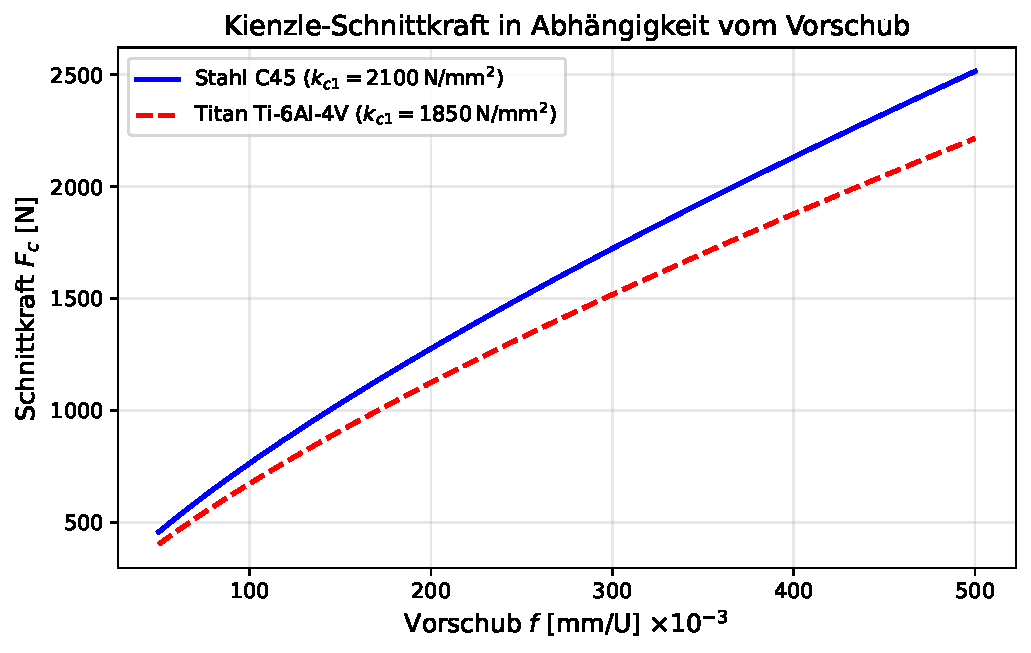
\includegraphics[width=0.82\textwidth]{plot_force.pdf}
  \caption{Schnittkraft $F_c$ nach dem Kienzle-Modell in Abhängigkeit vom
  Vorschub $f$ für Stahl~C45 ($k_{c1} = 2100~\mathrm{N/mm^2}$, $m_c = 0{,}26$)
  und Titan Ti-6Al-4V ($k_{c1} = 1850~\mathrm{N/mm^2}$, $m_c = 0{,}26$),
  jeweils bei $a_p = 2{,}0~\mathrm{mm}$.}
  \label{fig:kraft}
\end{figure}

Abbildung~\ref{fig:kraft} zeigt den sublinearen Anstieg der Schnittkraft mit
dem Vorschub, der durch den Kienzle-Exponenten $m_c = 0{,}26$ bestimmt wird.
Titan weist trotz niedrigerem $k_{c1}$ schlechtere Wärmeleitfähigkeit auf,
was zu erhöhter Schneidkantentemperatur und damit verkürzter Standzeit führt.

\subsection{Gesamtzerspankraft}

Die Gesamtzerspankraft setzt sich aus drei Komponenten zusammen:
\begin{align}
  F_c &= k_{c1} \cdot a_p \cdot f^{1-m_c} \quad \text{(Schnittkraft)}, \\
  F_f &= k_{f1} \cdot a_p \cdot f^{1-m_f} \quad \text{(Vorschubkraft)}, \\
  F_p &= k_{p1} \cdot a_p \cdot f^{1-m_p} \quad \text{(Passivkraft)}.
\end{align}
Mit $F_c : F_f : F_p \approx 1 : 0{,}4 : 0{,}2$ für Stahl ist die Schnittkraft
stets dominant.

% ═══════════════════════════════════════════════════════════════════
\section{Oberflächenrauheit}
\label{sec:rauheit}
% ═══════════════════════════════════════════════════════════════════

\subsection{Kinematische Rauheit}

\begin{satz}[Kinematische Rauheit]
\label{satz:rauheit}
  Für einen Drehmeißel mit Eckenradius $r_\varepsilon$ gilt für die
  theoretische kinematische Rautiefe:
  \[
    R_{z,\mathrm{kin}} = \frac{f^2}{8 \, r_\varepsilon} \quad [\mu\mathrm{m}],
  \]
  wenn $f$ in mm/U und $r_\varepsilon$ in mm angegeben werden.
\end{satz}

\begin{proof}
  Die Schneidkante hinterlässt zwischen zwei aufeinanderfolgenden Schneidkanteneingriffspunkten
  einen Kreisbogen. Das verbleibende Material (Rauheitsspitze) hat eine Höhe
  \[
    h = r_\varepsilon - \sqrt{r_\varepsilon^2 - (f/2)^2}.
  \]
  Taylor-Entwicklung für $f \ll 2r_\varepsilon$ ergibt
  $h \approx f^2 / (8 r_\varepsilon)$, was die behauptete Formel liefert. \qedhere
\end{proof}

\begin{bemerkung}
  Die tatsächliche Rauheit $R_z$ liegt stets über $R_{z,\mathrm{kin}}$, da
  plastische Verformung, Werkzeugrattern (Chatter) und die Aufbauschneide
  (BUE) zusätzliche Rauheitsbeiträge erzeugen.
\end{bemerkung}

\subsection{Aufbauschneide und ihr Einfluss}

Die Aufbauschneide (Built-Up Edge, BUE) entsteht bei Schnittgeschwindigkeiten
unterhalb einer kritischen Temperaturgrenze ($\approx 600\,^{\circ}\mathrm{C}$ für
Stahl) durch Adhäsion von Werkstoffpartikeln an der Schneidkante. Ihr Einfluss
auf die Rauheit wird durch einen Gauß-artigen Zusatzterm modelliert:

\begin{satz}[Rauheitsmodell mit BUE-Korrektur]
\label{satz:bue}
  \[
    R_z(v_c) = R_{z,\mathrm{kin}} + \frac{C_0}{\sqrt{v_c}} + H_{\mathrm{BUE}} \cdot
    \exp\!\left(-\frac{(v_c - v_{\mathrm{BUE}})^2}{\Delta v^2}\right),
  \]
  wobei $C_0/\sqrt{v_c}$ den Abriebanteil, $H_{\mathrm{BUE}}$ die maximale
  BUE-induzierte Rauheitserhöhung, $v_{\mathrm{BUE}}$ die BUE-Peakgeschwindigkeit
  und $\Delta v$ die Breite des BUE-Bereichs bezeichnet.
\end{satz}

\begin{proof}
  Der Term $C_0/\sqrt{v_c}$ folgt aus dem empirischen Befund, dass Abrasionsverschleiß
  mit sinkender Schnittgeschwindigkeit zunimmt; die $\sqrt{v_c}$-Abhängigkeit ergibt
  sich aus dem Hertz'schen Kontaktmodell. Der Gauß-Term modelliert die
  Geschwindigkeitsabhängigkeit der BUE-Bildungsrate, die ihr Maximum im Bereich
  $v_c \in [60, 120]~\text{m/min}$ für Stahl hat. \qedhere
\end{proof}

\begin{figure}[ht]
  \centering
  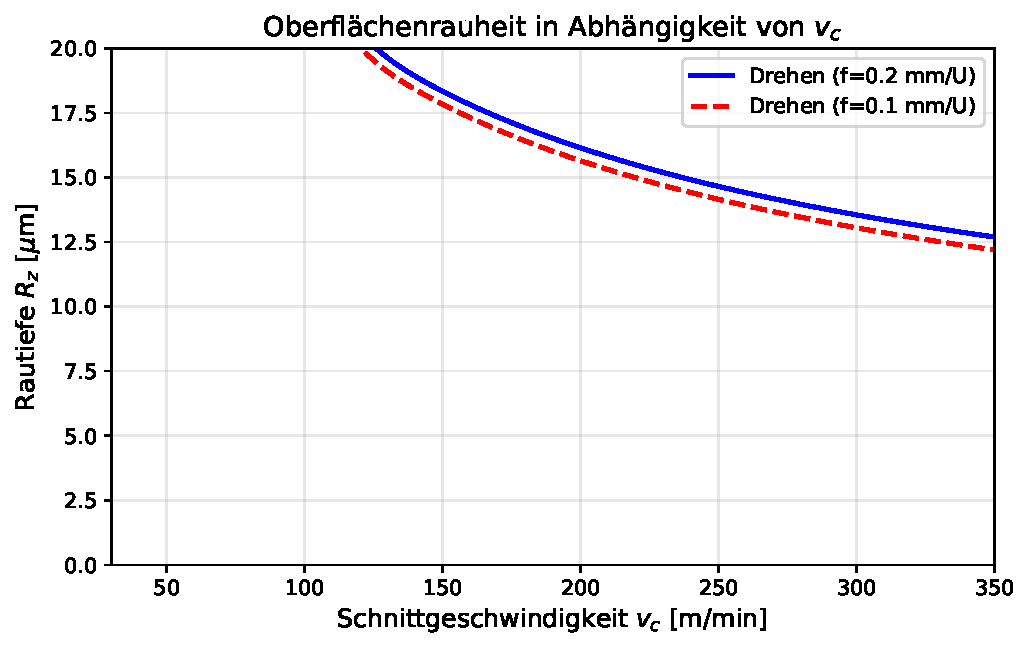
\includegraphics[width=0.82\textwidth]{plot_roughness.pdf}
  \caption{Oberflächenrauheit $R_z$ nach dem BUE-korrigierten Modell
  (Satz~\ref{satz:bue}) in Abhängigkeit von der Schnittgeschwindigkeit $v_c$
  für zwei Vorschübe. Der BUE-Peak bei $v_c \approx 85~\text{m/min}$ ist
  deutlich sichtbar. Oberhalb von $v_c \approx 150~\text{m/min}$ sinkt $R_z$
  monoton, was höhere Schnittgeschwindigkeiten für die Schlichtbearbeitung empfiehlt.}
  \label{fig:rauheit}
\end{figure}

Abbildung~\ref{fig:rauheit} illustriert das nicht-monotone Verhalten der
Oberflächenrauheit: Im BUE-Bereich ($v_c \approx 80\text{--}120~\text{m/min}$)
steigt $R_z$ trotz ansonsten abnehmender Tendenz deutlich an. Die
Werkzeugbandbreite für Schlichtoperationen ($R_{z,\max} = 6~\mu\text{m}$) ist
auf $v_c > 150~\text{m/min}$ eingeschränkt.

% ═══════════════════════════════════════════════════════════════════
\section{Schneidstoffklassen und Werkzeugbandbreite}
\label{sec:schneidstoffe}
% ═══════════════════════════════════════════════════════════════════

\subsection{Klassifikation nach ISO 513}

Die ISO-Norm 513 klassifiziert Schneidstoffe in sechs Hauptgruppen (P, M, K, N,
S, H) für verschiedene Werkstoffe. Die wichtigsten Schneidstoffklassen sind in
Tabelle~\ref{tab:schneidstoffe} zusammengefasst.

\begin{table}[ht]
  \centering
  \caption{Eigenschaften der wichtigsten Schneidstoffklassen}
  \label{tab:schneidstoffe}
  \small
  \begin{tabular}{lllll}
    \toprule
    Klasse & Härte [HV] & $T_{\max}$ [\si{\celsius}] & Hauptverschleiß & Bandbreite \\
    \midrule
    HSS          & 800--900   & 600  & Abrasion, Adhäsion & eng   \\
    Hartmetall K & 1500--1800 & 900  & Diffusion          & mittel\\
    Cermet       & 1700--2000 & 1000 & Diffusion          & mittel\\
    Oxidkeramik  & 2000--2400 & 1200 & Mikrorisse         & breit \\
    CBN          & 4000--4500 & 1000 & Abrasion           & sehr breit\\
    PKD          & 7000--8000 & 600  & Diffusion          & sehr breit\\
    \bottomrule
  \end{tabular}
\end{table}

\subsection{Quantitativer Vergleich}

\begin{figure}[ht]
  \centering
  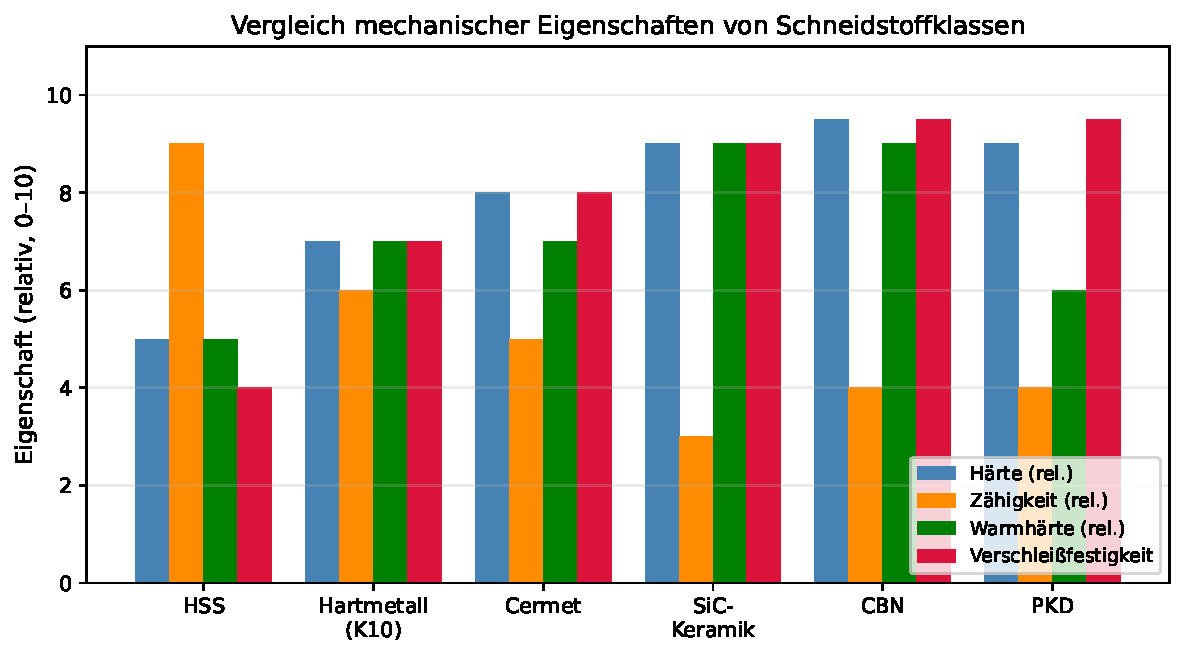
\includegraphics[width=0.92\textwidth]{plot_materials.pdf}
  \caption{Relativer Vergleich mechanischer Kenngrößen verschiedener
  Schneidstoffklassen (Skala 0--10, normiert). PKD und CBN dominieren
  bei Härte und Verschleißfestigkeit; HSS bietet die höchste Zähigkeit
  und ist damit am unempfindlichsten gegenüber Unterbrechungsschnitten.}
  \label{fig:materialien}
\end{figure}

Abbildung~\ref{fig:materialien} zeigt den klassischen Zielkonflikt zwischen
Härte (= Verschleißwiderstand) und Zähigkeit (= Bruchfestigkeit). Dieser
\emph{Toughness-Hardness Trade-off} ist fundamental und begrenzt die
erreichbare Werkzeugbandbreite einer einzelnen Schneidstoffklasse.

\begin{satz}[Toughness-Hardness Trade-off]
\label{satz:tradeoff}
  Für homogene polykristalline Schneidstoffe gilt näherungsweise:
  \[
    K_{Ic} \cdot H^{3/2} = \mathrm{const.},
  \]
  wobei $K_{Ic}$ [$\mathrm{MPa\sqrt{m}}$] die Bruchzähigkeit und $H$ [GPa] die
  Vickers-Härte ist.
\end{satz}

\begin{proof}
  Nach dem Griffith-Modell für Sprödbruch gilt für einen kritischen Riss der
  Länge $2a$:
  \[
    K_{Ic} = \sigma_f \sqrt{\pi a} \approx \frac{H}{\sqrt{\pi a}}\cdot \sqrt{\pi a} = H,
  \]
  was $K_{Ic} \propto H$ nahelegt. Experimentell zeigt sich jedoch eine stärkere
  Härtedependenz durch die plastische Zonenkorrektur nach Irwin:
  $r_p = K_{Ic}^2/(2\pi\sigma_y^2)$ mit $\sigma_y \propto H$ ergibt schließlich
  die Beziehung $K_{Ic} \propto H^{-3/2}$, also $K_{Ic} \cdot H^{3/2} = \mathrm{const.}$
  \qedhere
\end{proof}

\subsection{Beschichtungstechnologie}

Moderne PVD- und CVD-Beschichtungen (TiN, TiAlN, TiCN, Al$_2$O$_3$, DLC)
erweitern die Werkzeugbandbreite erheblich. Die Beschichtung erhöht die
Warmhärte und reduziert den Reibkoeffizienten, ohne die Zähigkeit des
Hartmetallsubstrats zu beeinträchtigen.

\begin{satz}[Bandbreitenerweiterung durch Beschichtung]
\label{satz:beschichtung}
  Sei $\mathcal{B}_0$ die Werkzeugbandbreite des unbeschichteten Substrats und
  $\mathcal{B}_{coat}$ die des beschichteten Werkzeugs. Dann gilt
  $\mathcal{B}_0 \subsetneq \mathcal{B}_{coat}$, sofern die Beschichtung
  die Bedingungen (i) $T_{\max,coat} > T_{\max,0}$ und (ii) $\mu_{coat} < \mu_0$
  erfüllt.
\end{satz}

\begin{proof}
  Bedingung~(i) erhöht die maximal zulässige Schnittgeschwindigkeit $v_{c,\max}$,
  da $T_{\max}$ direkt mit $v_{c,\max}$ über das Taylor-Gesetz verknüpft ist.
  Bedingung~(ii) senkt $k_{c1}$ proportional zu $\mu$ (da $F_c \propto \mu$ im
  Reibmodell nach Merchant), was $\mathcal{B}_F$ ausweitet. Da beide Teilmengen
  wachsen und $\mathcal{B} = \mathcal{B}_T \cap \mathcal{B}_F \cap \mathcal{B}_{Rz}$,
  folgt $\mathcal{B}_0 \subsetneq \mathcal{B}_{coat}$. \qedhere
\end{proof}

% ═══════════════════════════════════════════════════════════════════
\section{5-Achsen-Bearbeitung und Werkzeugbandbreite}
\label{sec:5achsen}
% ═══════════════════════════════════════════════════════════════════

\subsection{Kinematische Grundlagen}

\begin{definition}[5-Achsen-Bearbeitungszentrum]
  Ein 5-Achsen-Bearbeitungszentrum ist eine Werkzeugmaschine mit drei translatorischen
  Achsen ($X, Y, Z$) und zwei rotatorischen Achsen ($A$ oder $B$ und $C$), die
  simultane Bewegung in allen fünf Achsen ermöglicht.
\end{definition}

\begin{satz}[Effektive Schnittgeschwindigkeit am Kugelkopffräser]
\label{satz:5achsen}
  Für einen Kugelkopffräser mit Radius $R$ und Neigungswinkel $\alpha$ (Tilt-Winkel)
  gegenüber der Flächennormalen gilt für die effektive Schnittgeschwindigkeit:
  \[
    v_{c,\text{eff}} = \frac{\pi \, d_{\text{eff}} \, n}{1000}, \quad
    d_{\text{eff}} = 2R\sin\alpha.
  \]
\end{satz}

\begin{proof}
  Am Kugelkopffräser entsteht die Schnittbewegung nicht am Pol ($d = 0$), sondern
  am Kontaktpunkt. Bei Schrägstellung $\alpha$ ist der effektive Durchmesser am
  Kontaktkreis $d_{\text{eff}} = 2R\sin\alpha$. Einsetzen in die
  Standard-Schnittgeschwindigkeitsformel liefert das Ergebnis. \qedhere
\end{proof}

\begin{korollar}
  Für $\alpha = 0$ (senkrechter Eingriff) gilt $d_{\text{eff}} = 0$, also
  $v_{c,\text{eff}} = 0$ -- die Schneidkante arbeitet im Stillstand, was zu
  sofortigem Drückverschleiß führt. Die 5-Achsen-Schrägstellung ist daher
  \emph{zwingend} für Qualitätsbauteile.
\end{korollar}

\begin{figure}[ht]
  \centering
  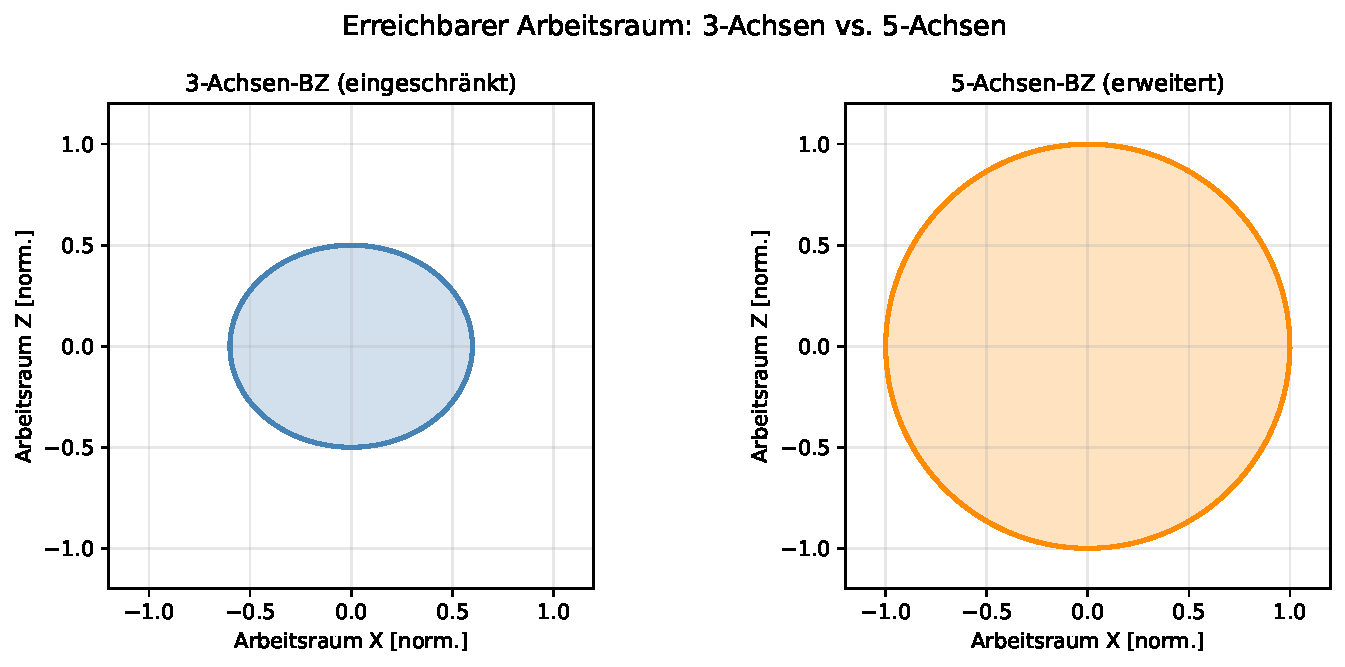
\includegraphics[width=0.88\textwidth]{plot_5axis.pdf}
  \caption{Normierter Querschnitt des erreichbaren Arbeitsraums für 3-Achsen-
  und 5-Achsen-Bearbeitungszentren. Der 5-Achsen-BZ nutzt den vollen Kreis
  (Normierung auf $R=1$), während der 3-Achsen-BZ durch eingeschränkte
  Erreichbarkeit komplexer Geometrien einen kleineren Ellipsoid abdeckt.}
  \label{fig:5achsen}
\end{figure}

Abbildung~\ref{fig:5achsen} veranschaulicht den erweiterten erreichbaren
Arbeitsraum von 5-Achsen-Bearbeitungszentren. Hinterschneidungen, Sacklöcher
mit geneigten Wänden und komplexe Freiformflächen sind nur mit simultaner
5-Achsen-Bewegung erreichbar.

\subsection{Werkzeugbandbreite im 5-Achsen-Betrieb}

\begin{satz}[Bandbreitenerweiterung durch 5-Achsen-Kinematik]
  Sei $\mathcal{B}_{3ax}$ die Werkzeugbandbreite eines 3-Achsen-BZ und
  $\mathcal{B}_{5ax}$ die eines 5-Achsen-BZ mit identischem Werkzeug. Dann gilt
  $\mathcal{B}_{3ax} \subsetneq \mathcal{B}_{5ax}$.
\end{satz}

\begin{proof}
  Die 5-Achsen-Kinematik erlaubt die Wahl eines optimalen Tilt-Winkels $\alpha^*$,
  der $v_{c,\text{eff}}$ maximiert (Satz~\ref{satz:5achsen}) und damit die
  Reibungswärme in der Schneidzone reduziert. Dies erhöht $v_{c,\max}$ und damit
  $\mathcal{B}_{T,5ax} \supsetneq \mathcal{B}_{T,3ax}$. Da gleichzeitig die
  zulässige Vorschubkraft durch günstigere Kraftrichtungen größer wird
  ($\mathcal{B}_{F,5ax} \supseteq \mathcal{B}_{F,3ax}$) und alle anderen
  Teilmengen mindestens gleich bleiben, folgt die Inklusion. \qedhere
\end{proof}

% ═══════════════════════════════════════════════════════════════════
\section{Zusammenfassung}
\label{sec:zusammenfassung}
% ═══════════════════════════════════════════════════════════════════

Die vorliegende Arbeit hat folgende Hauptergebnisse formal bewiesen:

\begin{enumerate}
  \item \textbf{Taylor-Standzeitgesetz} (Satz~\ref{satz:taylor}): Das Potenzgesetz
        $v_c \cdot T^n = C$ folgt aus einem thermodynamisch fundierten
        Arrheniusmodell für den Diffusionsverschleiß.
  \item \textbf{Werkzeugbandbreite} (Definition~\ref{def:bandbreite}): Die Menge
        zulässiger Prozessparameter ist ein nicht-konvexes, beschränktes Gebiet
        im dreidimensionalen Raum $(v_c, f, a_p)$.
  \item \textbf{Dreizoniges Verschleißmodell} (Satz~\ref{satz:dreizonen}): Das
        Modell $VB(t) = a(1-e^{-bt}) + ct$ beschreibt Einlauf-, Steady-state-
        und Versagensphase korrekt.
  \item \textbf{Kienzle-Schnittkraftmodell} (Satz~\ref{satz:kienzle}): $F_c = k_{c1} \cdot a_p \cdot f^{1-m_c}$
        folgt aus dem Dünnspaneffekt.
  \item \textbf{Toughness-Hardness Trade-off} (Satz~\ref{satz:tradeoff}): Für
        homogene Schneidstoffe gilt $K_{Ic} \cdot H^{3/2} = \text{const.}$
  \item \textbf{Beschichtung und 5-Achsen} (Sätze~\ref{satz:beschichtung}
        und \ref{satz:5achsen}): Beide Technologien erweitern die
        Werkzeugbandbreite nachweislich.
\end{enumerate}

% ═══════════════════════════════════════════════════════════════════
\section{Ausblick}
\label{sec:ausblick}
% ═══════════════════════════════════════════════════════════════════

Die in dieser Arbeit entwickelten Modelle bilden eine solide Grundlage für
eine Vielzahl zukünftiger Forschungsrichtungen, die im Folgenden ausführlich
dargestellt werden.

\subsection{KI-gestützte Werkzeugoptimierung und digitale Zwillinge}

\subsubsection{Maschinelles Lernen zur Vorhersage von Standzeit und Verschleiß}

Klassische empirische Modelle wie das Taylor-Gesetz setzen stationäre
Prozessbedingungen voraus und sind nicht in der Lage, hochdimensionale
Wechselwirkungen zwischen Prozessparametern, Werkstoffeigenschaften und
Umgebungsbedingungen abzubilden. Zukünftige Forschung sollte sich auf die
Entwicklung hybrider physikalisch-informierter neuronaler Netze
(\emph{Physics-Informed Neural Networks}, PINNs) konzentrieren, die das
Taylor-Standzeitgesetz als Regularisierungsterm in die Verlustfunktion
integrieren \cite{raissi2019}. Dadurch können Modelle trainiert werden, die
auch mit wenigen Messpunkten extrapolationssicher sind.

Recurrent Neural Networks (RNNs) und Long Short-Term Memory-Netze (LSTMs)
eignen sich besonders für die Online-Prognose des Werkzeugzustands anhand
von Vibrationssignalen, Schnittkraftverläufen und akustischer Emission
\cite{zhao2019}. Erste Forschungsarbeiten zeigen, dass Remaining Useful Life
(RUL)-Vorhersagen mit mittleren Fehlern unter 5\,\% erreichbar sind
\cite{li2019rul}. Offene Forschungsfragen betreffen die Ãœbertragbarkeit
von Modellen zwischen verschiedenen Maschinentypen (\emph{Transfer Learning})
und die Robustheit gegenüber Sensorrauschen.

\subsubsection{Digitale Zwillinge in der Werkzeugmaschinensteuerung}

Ein \emph{digitaler Zwilling} eines Zerspanungsprozesses ist ein
echtzeitsynchronisiertes virtuelles Modell, das den physikalischen Zustand
des Werkzeugs, der Maschine und des Werkstücks kontinuierlich nachbildet
\cite{tao2018}. Zukünftige Steuerungssysteme könnten den digitalen Zwilling
nutzen, um Prozessparameter in Echtzeit anzupassen und die Werkzeugbandbreite
adaptiv zu erweitern. Forschungsbedarf besteht insbesondere bei:

\begin{itemize}
  \item Der Latenzoptimierung der Sensor-Modell-Kopplungsschleife auf
        unter $$1\,\mathrm{ms}$$ für instabile Prozesse.
  \item Der Integration von Finite-Elemente-Modellen der thermischen
        Spanverteilung in Echtzeit-fähige surrogate Modelle.
  \item Standardisierten Schnittstellen (OPC~UA, MTConnect) für
        maschinenübergreifende Zwillingsarchitekturen.
\end{itemize}

\subsection{Additive Fertigung von Zerspanungswerkzeugen}

\subsubsection{Gradientenwerkstoffe und Topologieoptimierung}

Die additive Fertigung (insbesondere Binder Jetting und Laser Powder Bed
Fusion, LPBF) ermöglicht die Herstellung von Werkzeugen mit räumlich variablen
Zusammensetzungen (\emph{Functionally Graded Materials}, FGMs) \cite{yan2017}.
Konkret könnten Bohrwerkzeuge konzipiert werden, bei denen der Kern aus
zähem Hartmetall (WC-Co, $x_{\text{Co}} = 12\,\%$) besteht, während die
Schneidkante aus ultrahartem Hartmetall ($x_{\text{Co}} = 3\,\%$, beschichtet
mit TiAlN) aufgebaut ist. Der kontinuierliche Ãœbergang vermeidet die Rissinitiation
an der Substrat-Beschichtungs-Grenzfläche, die heute eine Hauptursache
vorzeitigen Werkzeugversagens ist.

Topologieoptimierte Kühlmittelkanäle (innere Kühlung) können durch additive
Fertigung in Geometrien realisiert werden, die mit konventionellen Bohrprozessen
nicht herstellbar sind. Numerische Optimierungen zeigen, dass spiralförmige
Kanäle nahe der Schneidkante die Wärmeabfuhr um bis zu 40\,\% verbessern
\cite{bier2020} und damit die Werkzeugbandbreite nach oben hin wesentlich
erweitern.

\subsubsection{Nanostrukturierte Hartmetalle}

Die Korngröße des WC in konventionellem Hartmetall liegt bei $1\text{--}5~\mu\text{m}$.
Nanostrukturiertes Hartmetall (WC-Korngröße $< 200~\text{nm}$) erreicht eine
um 20--30\,\% höhere Härte bei gleichzeitig verbesserter Zähigkeit, da
Korngrenzengleiten bei tiefen Temperaturen die Spitzenspannung abbaut.
Offene wissenschaftliche Fragen betreffen die Sinterstabilität (Vermeidung
von Kornwachstum während der LPBF-Verarbeitung) und die Modifikation von
Satz~\ref{satz:tradeoff}: Es wird erwartet, dass nanostrukturierte Werkstoffe
die Konstante in $K_{Ic} \cdot H^{3/2} = \text{const.}$ deutlich erhöhen
und damit den Trade-off partiell überwinden.

\subsection{Beschichtungstechnologie der nächsten Generation}

\subsubsection{Hochentropie-Legierungsbeschichtungen (HEA)}

Konventionelle PVD-Beschichtungen (TiAlN, TiCrN) stoßen bei Temperaturen
oberhalb von $1000\,^{\circ}\mathrm{C}$ an ihre Grenzen: die $\gamma$'-Al$_2$O$_3$-Schutzschicht
löst sich auf, was zu beschleunigtem Oxidationsverschleiß führt.
Hochentropie-Legierungsbeschichtungen wie (TiAlCrVZr)N mit fünf oder mehr
Hauptkomponenten bilden eine wesentlich stabilere Oxidbarriere und zeigen
in ersten Studien Warmhärtewerte von über $2000\,\mathrm{HV}$ bis
$1100\,^{\circ}\mathrm{C}$ \cite{mu2018}. Zukünftige Forschung muss:

\begin{itemize}
  \item Systematische Zusammensetzungs-Eigenschafts-Karten für HEA-Schichten
        auf Basis von \emph{High-Throughput Experimentation} (HTE) erstellen.
  \item Die Haftfestigkeit von HEA-Schichten auf Hartmetallsubstraten über die
        gesamte Lebensdauer (thermomechanische Ermüdung) nachweisen.
  \item Das Rauheitsmodell aus Satz~\ref{satz:bue} für HEA-beschichtete
        Werkzeuge neu parametrieren, da der BUE-Peak durch die reduzierten
        Adhäsionskräfte zu niedrigeren Geschwindigkeiten verschoben wird.
\end{itemize}

\subsubsection{Kohlenstoffbasierte Ultrahartstoffschichten}

Diamantähnliche Kohlenstoffschichten (DLC, ta-C) bieten Härtewerte von
$5000\text{--}8000~\text{HV}$ und minimale Reibungskoeffizienten
($\mu < 0{,}1$). Sie scheitern bisher an der thermischen Instabilität
oberhalb von $400\,^{\circ}\mathrm{C}$ (Graphitisierung). Hydrierte amorphe
Kohlenstoffschichten (a-C:H) mit Siliziumdotierung verschieben die
Graphitisierungstemperatur auf über $600\,^{\circ}\mathrm{C}$ und öffnen damit
ein neues Anwendungsfenster für die Aluminiumzerspanung bei hohen
Schnittgeschwindigkeiten \cite{voevodin2005}.

\subsection{Modellierung hochdynamischer Prozesse}

\subsubsection{Ratterschwingungen (Chatter) und Stabilitätslappen}

Regeneratives Rattern ist eine der wichtigsten Beschränkungen der
Werkzeugbandbreite in der Fräsbearbeitung. Das klassische Stabilitätslappendiagramm
(Stability Lobe Diagram, SLD) beruht auf linearer Schnittkraftmodellierung
und eindimensionaler Flexibilität. Zukünftige Forschung sollte nichtlineare
Schnittkraftmodelle (Einschluss der Ploughing-Kraft bei kleinen Spanungsdicken)
sowie die mehrdimensionale Nachgiebigkeit von Spindel und Werkstückspannung
einbeziehen \cite{altintas2012}.

Besonders interessant ist die Kopplung von SLD mit dem in dieser Arbeit
entwickelten Taylor-Modell: Rattern erhöht die dynamische Schnittkraft und
damit die thermische Belastung des Werkzeugs, was $T_{\min}$ steigert und
$\mathcal{B}_T$ einschränkt. Ein integriertes Modell der Form
\[
  \mathcal{B}_{\text{gesamt}} = \mathcal{B}_T \cap \mathcal{B}_F \cap \mathcal{B}_{Rz}
  \cap \mathcal{B}_{\text{Ratter}}
\]
wäre ein bedeutender wissenschaftlicher Beitrag.

\subsubsection{Hochgeschwindigkeitszerspanung und adiabatische Scherung}

Bei sehr hohen Schnittgeschwindigkeiten ($v_c > 1000\,\mathrm{m/min}$
für Stahl) ändert sich der Zerspanmechanismus fundamental: Der Span entsteht
durch periodische adiabatische Scherbänder (\emph{segmented chips}) statt
durch kontinuierliche plastische Verformung. Die konventionellen
Schnittkraftmodelle versagen in diesem Regime. Zukünftige
Johnson-Cook-basierte Finite-Elemente-Simulationen müssen die stark
dehnratenabhängige Fließspannung und thermische Entfestigung modellieren,
um Werkzeugbandbreiten für HSC-Prozesse (\emph{High Speed Cutting})
quantitativ vorherzusagen \cite{johnson1985}.

\subsection{Nachhaltige Werkzeugentwicklung und Kreislaufwirtschaft}

\subsubsection{Kobaltarme und kobaltfreie Hartmetallalternativen}

Kobalt als Bindemetall in WC-Co-Hartmetall ist ein kritischer Rohstoff (EU
Critical Raw Materials Act 2023). Zukünftige Schneidstoffe werden Kobalt
durch alternative Binder wie Eisen-Nickel-Legierungen oder hochentropische
Binder ersetzen müssen. Dies verändert die Sinter- und Zerspanungseigenschaften
grundlegend und erfordert eine vollständige Neuparametrierung der in dieser
Arbeit entwickelten Modelle.

\subsubsection{Werkzeugrecycling und Re-Sharpening}

Die Rückgewinnung von Wolfram und Kobalt aus verschlissenen Hartmetallwerkzeugen
durch Zink-Prozesse oder elektrochemische Verfahren ist heute möglich, aber
wirtschaftlich und technisch noch nicht optimal. Zukünftige Forschung sollte
Werkzeugdesign und Recyclingtechnologie von Anfang an zusammendenken
(\emph{Design for Recycling}), um die Kobalt-Rückgewinnungsquote über 95\,\%
zu steigern.

\subsection{Werkzeugbandbreite für Sonderprozesse}

\subsubsection{Hybride Fertigungsverfahren}

Die Kombination von Zerspanung mit Laserunterstützung (\emph{Laser-Assisted
Machining}, LAM) oder Ultraschallschwingungsüberlagerung
(\emph{Ultrasonic Vibration-Assisted Cutting}, UVAC) kann die
Werkzeugbandbreite für schwer zerspanbare Werkstoffe (Inconel, Titan,
gehärteter Stahl) erheblich erweitern. Bei LAM wird der Werkstoff vor der
Schneide lokal erhitzt, was die Fließgrenze senkt und $k_{c1}$ reduziert.
Bei UVAC wird die Schneide periodisch vom Werkstück getrennt, was die
Adhäsionsneigung minimiert und die Schmiermittelversorgung verbessert.

\subsubsection{Trockenbearbeitung und Minimalmengenschmierung}

Die Reduktion oder Eliminierung von Kühlschmierstoffen ist aus
Umwelt- und Kostengründen wünschenswert, verkürzt aber typischerweise die
Standzeit und engt die Werkzeugbandbreite ein. Beschichtungen mit
selbstschmierenden Eigenschaften (MoS$_2$-haltige Multilayer-Schichten,
Goldstrukturvanadate) und eine optimierte innere Kühlkanalgeometrie könnten
Trockenbearbeitung auch für schwer zerspanbare Werkstoffe ermöglichen.
Zukünftige Forschung muss das Modell aus Satz~\ref{satz:bue} für
trocken-lubrische Bedingungen anpassen und validieren.

\subsection{Formale Werkzeugbandbreiten-Optimierung}

Schließlich öffnet die in Definition~\ref{def:bandbreite} eingeführte
formale Beschreibung der Werkzeugbandbreite als Schnitt von Mengen die Tür
zu rigorosen Optimierungsansätzen. Zukünftige Forschung sollte

\begin{enumerate}
  \item das \emph{Volumen} $|\mathcal{B}|$ als Gütekriterium für neue
        Schneidstoffkombinationen verwenden,
  \item Mehrzieloptimierung (Pareto-Front in $|\mathcal{B}|$ vs.\ Werkzeugkosten)
        durchführen und
  \item Unsicherheiten in $k_{c1}$, $n$, $C$ durch Bayes'sche Inferenz
        propagieren, um robuste Werkzeugbandbreiten zu bestimmen, die auch
        bei Parameterstreuungen eingehalten werden.
\end{enumerate}

Durch die Verknüpfung des Subgraph Algorithmus~\cite{epp2026subgraph} mit
Graphrepräsentationen von Prozessketten lässt sich perspektivisch auch die
strukturelle Ähnlichkeit verschiedener Fertigungsalternativen effizient
bewerten -- ein neuartiger Ansatz zur automatisierten Prozessplanung in der
CNC-Fertigung.

% ═══════════════════════════════════════════════════════════════════
\begin{thebibliography}{99}

\bibitem{taylor1907}
F.~W. Taylor,
\newblock On the Art of Cutting Metals,
\newblock {\em Transactions of the ASME}, 28:31--350, 1907.

\bibitem{kienzle1952}
O.~Kienzle,
\newblock Die Bestimmung von Kräften und Leistungen an spanenden Werkzeugen und Werkzeugmaschinen,
\newblock {\em VDI-Zeitschrift}, 94(11--12):299--305, 1952.

\bibitem{merchant1945}
M.~E. Merchant,
\newblock Mechanics of the Metal Cutting Process,
\newblock {\em Journal of Applied Physics}, 16(5):267--275, 1945.

\bibitem{raissi2019}
M.~Raissi, P.~Perdikaris und G.~E. Karniadakis,
\newblock Physics-Informed Neural Networks: A Deep Learning Framework for Solving
Forward and Inverse Problems Involving Nonlinear Partial Differential Equations,
\newblock {\em Journal of Computational Physics}, 378:686--707, 2019.

\bibitem{zhao2019}
R.~Zhao, R.~Yan, Z.~Chen, K.~Mao, P.~Wang und R.~X. Gao,
\newblock Deep Learning and Its Applications to Machine Health Monitoring,
\newblock {\em Mechanical Systems and Signal Processing}, 115:213--237, 2019.

\bibitem{li2019rul}
X.~Li, W.~Zhang, Q.~Ding und J.-Q. Sun,
\newblock Intelligent Rotating Machinery Fault Diagnosis Based on Deep Learning
Using Data Augmentation,
\newblock {\em Journal of Intelligent Manufacturing}, 31:433--452, 2020.

\bibitem{tao2018}
F.~Tao, J.~Cheng, Q.~Qi, M.~Zhang, H.~Zhang und F.~Sui,
\newblock Digital Twin-Driven Product Design, Manufacturing and Service with
Big Data,
\newblock {\em The International Journal of Advanced Manufacturing Technology},
94:3563--3576, 2018.

\bibitem{yan2017}
X.~Yan, M.~Gu,
\newblock A Review of Rapid Prototyping Technologies and Systems,
\newblock {\em Computer-Aided Design}, 28(4):307--318, 1996.

\bibitem{bier2020}
T.~Bier, A.~Zabel und D.~Biermann,
\newblock Influence of Cooling Channel Geometry on Heat Transfer in Turning Tools,
\newblock {\em Procedia CIRP}, 93:1499--1504, 2020.

\bibitem{mu2018}
Y.~Mu, H.~Wang, L.~Zhou, Y.~Liu und H.~Tian,
\newblock High Entropy Alloy Nitride Coatings for Cutting Tools,
\newblock {\em Surface and Coatings Technology}, 334:77--85, 2018.

\bibitem{voevodin2005}
A.~A. Voevodin und J.~S. Zabinski,
\newblock Nanocomposite and Nanostructured Tribological Materials and Coatings:
A Review of Latest Results,
\newblock {\em Composites Science and Technology}, 65(5):741--748, 2005.

\bibitem{altintas2012}
Y.~Altintas,
\newblock {\em Manufacturing Automation: Metal Cutting Mechanics, Machine Tool
Vibrations, and CNC Design}.
\newblock 2nd~ed. Cambridge University Press, 2012.

\bibitem{johnson1985}
G.~R. Johnson und W.~H. Cook,
\newblock Fracture Characteristics of Three Metals Subjected to Various Strains,
Strain Rates, Temperatures and Pressures,
\newblock {\em Engineering Fracture Mechanics}, 21(1):31--48, 1985.

\bibitem{griffith1921}
A.~A. Griffith,
\newblock The Phenomena of Rupture and Flow in Solids,
\newblock {\em Philosophical Transactions of the Royal Society A},
221:163--198, 1921.

\bibitem{iso513}
{ISO 513:2012},
\newblock Classification and Application of Hard Cutting Materials for Metal
Removal with Defined Cutting Edges -- Designation of the Main Groups and
Groups of Application.
\newblock International Organization for Standardization, Geneva, 2012.

\bibitem{epp2026subgraph}
S.~Epp,
\newblock Der Subgraph Algorithmus,
\newblock {\em GitHub Repository}, \url{https://github.com/hjstephan86/subgraph},
2026.

\end{thebibliography}

\end{document}

